\subsubsection{Design Approach}
We have chosen to use the Customer Insight\cite{1} technique in our design approach. If we had the funds available, we could hire social scientists which could sketch profiles of the customer segment. As this is not the case, we have made use of the Empathy Map, which is also known as the ``really simple customer profiler''\cite{2}.

The first thing to do when using the empathy map, is to brainstorm all possible customer segments that one might want to serve with the business model. Then three promising candidates should be chosen, from which a single candidate is selected for the first profiling exercise. Then a customer from that customer segment is thought up, by giving the customer characteristics, such as a name, income, occupation, and so on. Afterwards a profile is build for the customer by asking and answering six questions.
These questions should be put on a white board or flip chart, as seen in figure \ref{fig:empathy_map}(Hence, empathy map), and the answers could be written on stick-it notes and placed on the questions.

The six questions are\cite{2}:
\begin{itemize}
\item What does the customer see? Describe what the customer sees in their environment
\item What does the customer hear? Describe how the environment influences the customer
\item What does the customer really feel and think? Try to sketch out what goes on in their mind
\item What does the customer say and do? Imagine what the customer might say, or how the customer might behave in public
\item What is the customer's pain? E.g. what are their biggest frustrations?
\item What does the customer gain? E.g. what does the customer truly want or need to achieve?
\end{itemize}

\begin{figure}[h]
    \begin{center}
        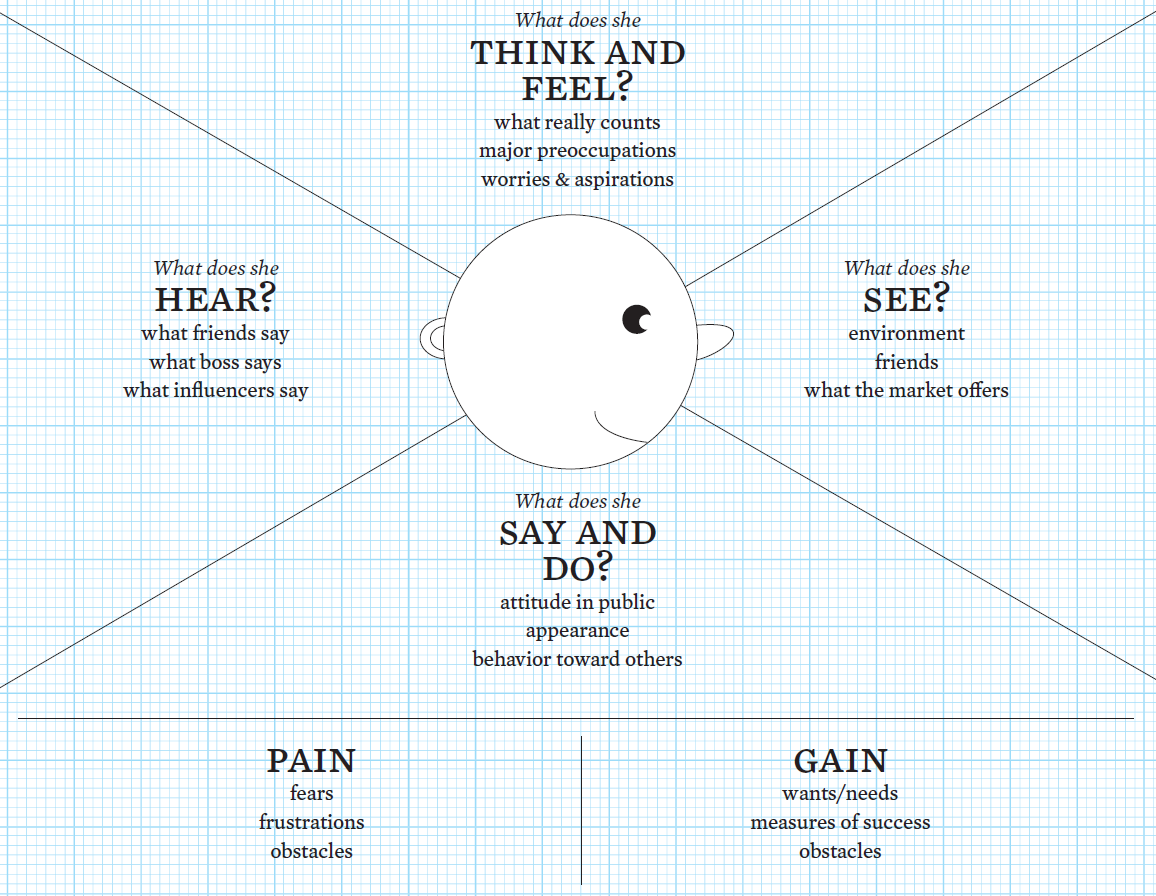
\includegraphics[scale=0.52]{./pics/empathy_map}
        \label{fig:empathy_map}
        \caption{Adapted empathy map from XPLANE\cite{3}}
    \end{center}
\end{figure}

The three candidate costumer segments we have come up with are:
\begin{enumerate}
\item Couples in the age range of 25-35, with children, that is ``forced'' to have cable because the children need their Saturday morning cartoons.
\item Students in the age range of 18-24, not living at home, limited income e.g. support from the government. Illegally downloads movies and TV-shows, as they can't afford cable or to buy them.
\item People in the age range of 16-35, illegally downloads movies and TV-shows because of ease-of-access.
\end{enumerate}

We are basing our customer on candidate 2 from the list. He is called John, he has no income except for support from the government, he is studying computer science at a university, he is single.

Question 1, what does he see?
\begin{itemize}
\item He lives in a small, one bedroom, apartment with no space for a TV
\item He is mostly surrounded by friends, as his family lives a couple of hours away, but will come visit occasionally 
\item His friends are people with similar interests as him self or study buddies, such as computers, video games, books and comics, TV shows and movies
\item He is not exposed to many offers in his daily routine, as he gets no advertisements from not owning a TV and he uses an ad blocker when surfing the internet
\end{itemize}

Question 2, what does he hear?
\begin{itemize}
\item His friends talk mostly about their shared interests
\item He is influenced by his friends and the internet, e.g. forums
\item He is not influenced by a lot of media channels, as he do not watch advertisements, and he do not visit social media often because people fills his wall with random games.
\item The most influential media channel is probably YouTube, where he gets the news he is interested in
\end{itemize}

Question 3, what does he really think and feel?
\begin{itemize}
\item \todo{I need help with what to put here, business model generation 131:Henrik}
\item He really want to be a video game developer
\end{itemize}

Question 4, what does he say and do?
\begin{itemize}
\item He has a friendly attitude in public, e.g. holding doors for people if necessary
\item He will mostly discuss ideas, talk about hobbies and so on
\item He enjoys a good discussion, does not have to be about anything, and he indulge in a little bit of gossiping 
\end{itemize}

Question 5, what is his pain?
\begin{itemize}
\item One of his biggest frustrations are having a hard time understanding a study related subject
\item An obstacle he faces, is that when he needs a break from studying, he watches an episode from a TV show, but keep watching more episodes because it is easier than studying
\end{itemize}

Question 6, what do he gain?
\begin{itemize}
\item \todo{I need help with what to put here, business model generation 131:Henrik}
\end{itemize}
% 1: Business model generation, 127-133
% 2: Business model generation, 131
% 3: Business model generation, 130